%%% Intro.tex --- 
%% 
%% Filename: Intro.tex
%% Description: 
%% Author: Ola Leifler
%% Maintainer: 
%% Created: Thu Oct 14 12:54:47 2010 (CEST)
%% Version: $Id$
%% Version: 
%% Last-Updated: Thu May 19 14:12:31 2016 (+0200)
%%           By: Ola Leifler
%%     Update #: 5
%% URL: 
%% Keywords: 
%% Compatibility: 
%% 
%%%%%%%%%%%%%%%%%%%%%%%%%%%%%%%%%%%%%%%%%%%%%%%%%%%%%%%%%%%%%%%%%%%%%%
%% 
%%% Commentary: 
%% 
%% 
%% 
%%%%%%%%%%%%%%%%%%%%%%%%%%%%%%%%%%%%%%%%%%%%%%%%%%%%%%%%%%%%%%%%%%%%%%
%% 
%%% Change log:
%% 
%% 
%% RCS $Log$
%%%%%%%%%%%%%%%%%%%%%%%%%%%%%%%%%%%%%%%%%%%%%%%%%%%%%%%%%%%%%%%%%%%%%%
%% 
%%% Code:


\chapter{Introduction}
\label{cha:introduction}

In this chapter, background and the goal of this project will be presented. 

\section{Motivation}
\label{sec:motivation}

%\cite{scigen}

% This is where the studied problem is described from a general
% point of view and put in a context which makes it clear that
% it is interesting and well worth studying. The aim is to make
% the reader interested in the work and create an urge to
% continue reading.

For years, robotics has been an active topic in lab environments and is now entering real human environments by helping humans with dangerous, repetitive and boring labour. A large part of the processes in industries are today executed by robots having higher speed and precision than humans. Autonomous vacuum cleaners and robot lawn mowers are today easy accessible in common stores. The next step is to make robots clean more complex environments such as streets and parking garages. A big challenge is to efficiently handle big environments and make plans over multiple floors. 

A company in Linköping, Dyno Rorobtics, is currently developing an autonomous sweeping robot. The aim of the robot is to clean streets, parking garages, parks and other outdoor environments. A fully working robot contains many components that have different importance depending on its application. For a sweeping robot one of the most important components is the path planning. Given data about the environment from the sensors the robot has to be able to plan a path that covers all accessible areas in the environment. Making a good plan that covers the whole area is of big importance. Upon missed spots, the robot has to clean a place more than once, making it less efficient.

The problem of planning a path that covers a region of interest while avoiding obstacles is called the Coverage Path Planning (CPP) problem. The CPP problem for flat surfaces is a well studied problem with established solutions. CPP algorithms solving the problem in 3D by covering areas on different heights, on the other hand, is harder and has many different approaches with different advantages. Simple 2D approaches are limited to cover only planes. These could be used in terrains with small inclination variations if the environment is still possible to represent as a 2D grid. This is not possible in environments with multiple floors and passages between them.  To handle this case, which is common in cities, CPP algorithms that handles a 3D representation of the environment are essential. \cite{mattiassurvey} 

This is the case in a multi floor parking garage with inclined roads, see Figure \ref{fig:parking_garage}. A CPP algorithm that covers a plane could be used separately on each floor, but would require a transformation of the area representation, because a bird view perspective is not enough to handle the inclined floor. The problem is illustrated in Figure \ref{fig:2dproblem}. Assuming that the road is horizontal is wrong since the range of the robot seen from the bird view will be smaller if the road is inclined. Consequently, a plan that neglects the inclination will result in missed regions. If a CPP algorithm that takes the height into consideration was used instead, there would be no need for the separation of the floors and the transformation of the area representation.

\begin{figure}
    \centering
    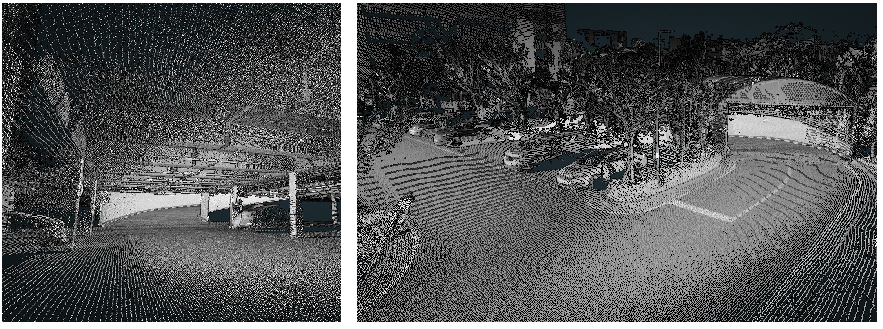
\includegraphics{figures/environment.pdf}
    \caption{A two-floor parking garage with inclined road. The area shown to the left is above the area to the right. The mission of the sweeper robot is to plan a path and clean both these floors.}
    \label{fig:parking_garage}
\end{figure}

\begin{figure}
    \centering
    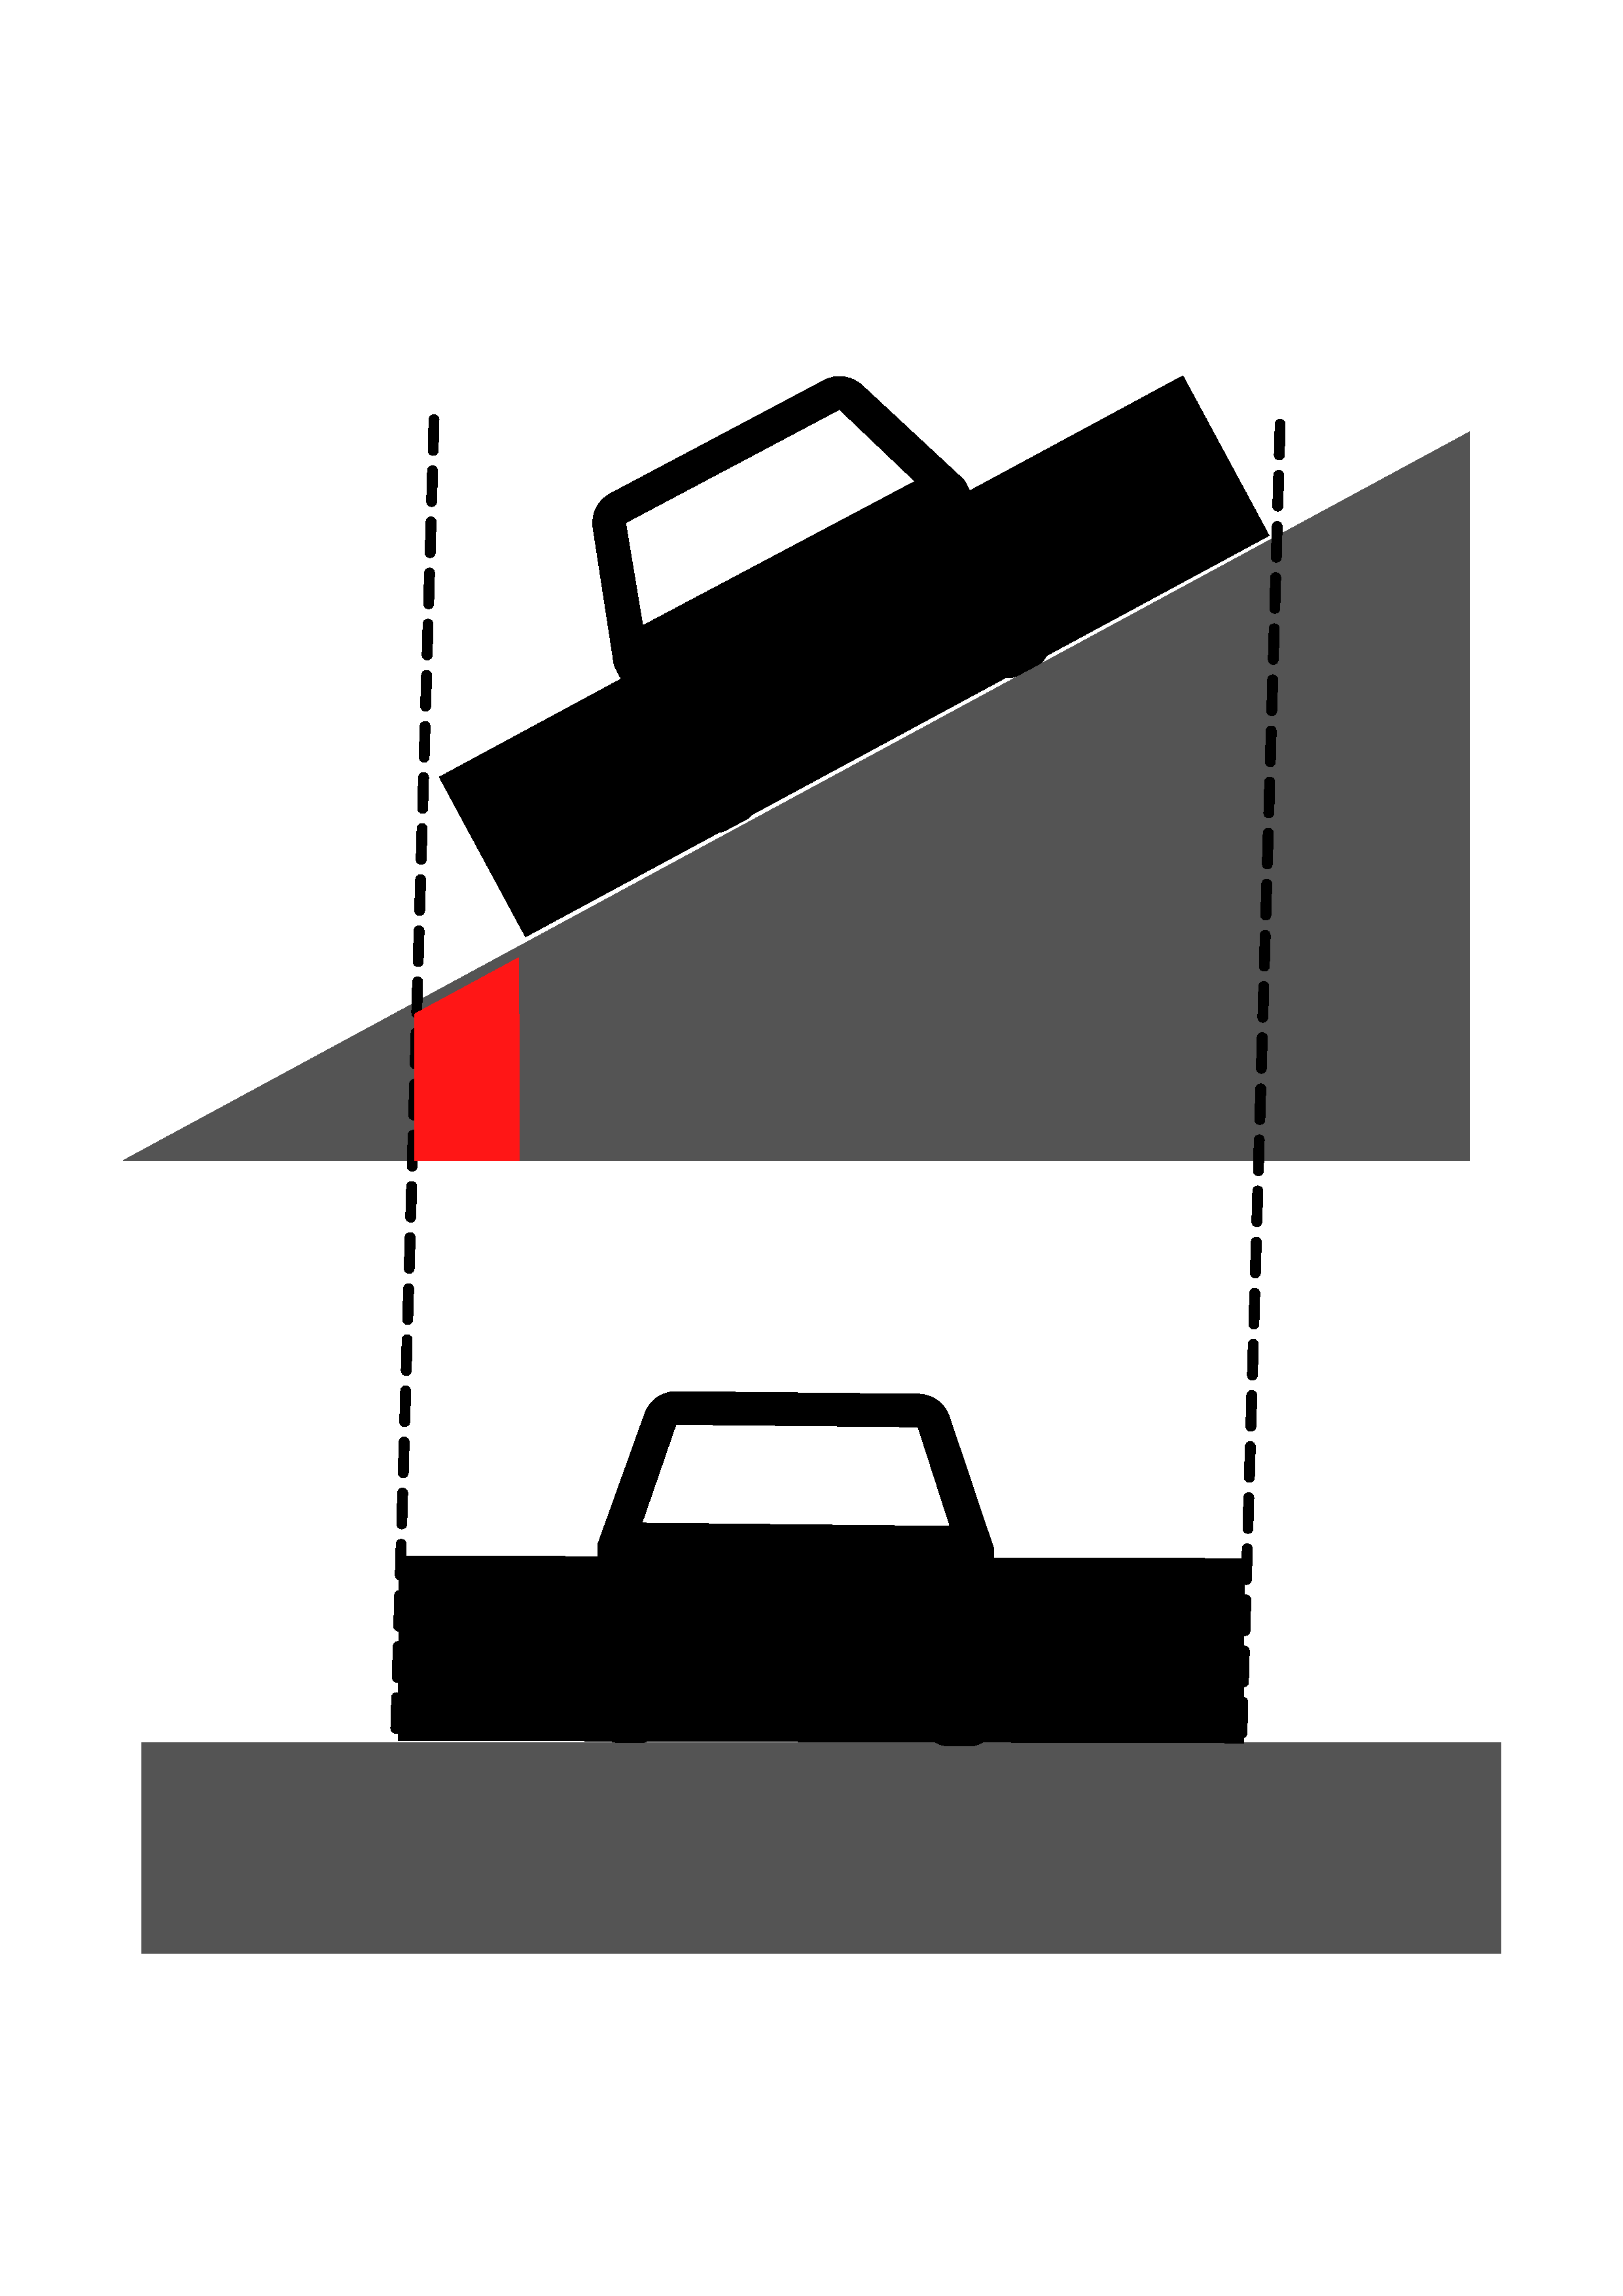
\includegraphics[width=0.4\textwidth]{figures/design.pdf}
    \caption{Neglecting the inclination of the ground results in skipped area. The range of the sweeper from a bird view perspective is smaller than expected.}
    \label{fig:2dproblem}
\end{figure}

The technology evolution has resulted in today's accessibility of sensors that are good enough for navigation of robots in 3D. According to business leaders autonomous vehicles are expected to be driving on our streets and do different tasks in complex environments in just a few years \cite{expertsai}. To solve the CPP problem in environments with multiple floors and height variations is today more important then ever and will make robots do tasks, where simple algorithms are insufficient.


% The expected result of the first part of this thesis is a comparison between a popular open source solution named OctoMap and a newer solution presented a few years ago, which makes this classification without discretizing the point cloud. Based on read literature an advantage of the OctoMap is it's compression ability making it less memory consuming. However, it could be more time consuming than the point cloud approach, because of the discretization.   

% The second part will present a 3D coverage path planning algorithm which could handle inclined floor in the parking garage better than today's 2D solution. Hopefully it will be able to plan for a coverage efficiency of close to 100\%. 


\section{Aim}
\label{sec:aim}


%What is the underlying purpose of the thesis project?

Today's path planning algorithm of Dyno Robotics sweeping robot is assuming that the terrain is flat. Since this is not the case for many of it's applications they need an effective 3D path planning solution that could handle more complicated environments. The aim of this thesis is to compare different methods and find the best way to solve this 3D CPP problem. 



\section{Research questions}
\label{sec:research-questions}

The input data for this problem will be a given 3D point cloud of a parking garage and the solution will be a path with waypoints in 3D. At least two steps will be needed. At first, traversible areas in the environment will be classified to know what areas should be cleaned. Secondly, this information will be given to an algorithm, which returns the solution path. This project will focus on the latter part by evaluating these questions:


% This is where the research questions are described.
% Formulate these as explicit questions, terminated with a
% question mark. A report will usually contain several different
% research questions that are somehow thematically connected.
% There are usually 2-4 questions in total.

% Examples of common types of research questions (simplified
% and generalized):

\begin{enumerate}
% \item How does technique X affect the possibility of achieving the
%   effect Y?

% \item How can a system (or a solution) for X be realized so
%   that the effect Y is achieved?

% \item What are the alternatives to
%   achieving X, and which alternative gives the best effect considering
%   Y and Z? (This research question is normally broken down in to 2
%   separate questions.)

%\item How much coverage effectiveness of a multi floor parking garage environment could be achieved if a robot follows a planned path? 

%\item Which 3D CPP algorithm has the best efficiency for the same amount of covered area in a multi floor parking garage environment?

\item How does coverage, length of path and total rotation change over time when planning a path to cover a multi floor outdoor environment using the algorithms Inward Spiral and BA*.

\item How does coverage, length of path and rotation changes when changing the priority order in BA*?

\item  Which algorithm, Inward Spiral, BA* or Curved BA*, is more suitable for autonomous covering regarding computational time, length of path and total rotation?

\item Can both the length of path and total rotation be improved with a sampling based method while keeping the coverage and computational time on the same level as Inward Spiral and BA*?

\end{enumerate}


% Observe that a very specific research question almost always
% leads to a better thesis report than a general research question
% (it is simply much more difficult to make something good
% from a general research question.)

% The best way to achieve a really good and specific research
% question is to conduct a thorough literature review and get
% familiarized with related research and practice. This leads to
% ideas and terminology which allows one to express oneself
% with precision and also have something valuable to say in the
% discussion chapter. And once a detailed research question
% has been specified, it is much easier to establish a suitable
% method and thus carry out the actual thesis work much faster
% than when starting with a fairly general research question. In
% the end, it usually pays off to spend some extra time in the
% beginning working on the literature review. The thesis
% supervisor can be of assistance in deciding when the research
% question is sufficiently specific and well-grounded in related
% research.

\section{Delimitations}
\label{sec:delimitations}

% This is where the main delimitations are described. For
% example, this could be that one has focused the study on a
% specific application domain or target user group. In the
% normal case, the delimitations need not be justified.

%\nocite{scigen}
%We have included Paper \ref{art:scigen}

The comparisons between the CPP algorithms will only be made on a point cloud of an underground parking garage in Daejeon, South Korea  \cite{jeong2019complex}. This point cloud is assumed to be given and all calculations are made offline. This project assumes that the robot follows the planned path exactly and count an area as cleaned if the robot's footprint has covered it at some point. 

%%%%%%%%%%%%%%%%%%%%%%%%%%%%%%%%%%%%%%%%%%%%%%%%%%%%%%%%%%%%%%%%%%%%%%
%%% Intro.tex ends here


%%% Local Variables: 
%%% mode: latex
%%% TeX-master: "demothesis"
%%% End: 
